
\documentclass{beamer}
\title{\textbf{CS251 Project Presentation}\\ \large by Group 25}   

%\author{Sohum Dhar \\{140070001@iitb.ac.in}, Himanshu Payal %\\{140050011@iitb.ac.in}, Aakash Praliya \\{140050012@iitb.ac.in}} 
\author[Sohum \& Himanshu \& Aakash]
{%
  \texorpdfstring{
    \begin{columns}%[onlytextwidth]
      \column{.30\linewidth}
      \centering
      Sohum Dhar\\
      \emph{140070001\\
      \href{mailto:140070001@iitb.ac.in}{140070001@iitb.ac.in}}
      \column{.30\linewidth}
      \centering
      Himanshu Payal\\
      \emph{140050011\\
      \href{mailto:140050011.iitb.ac.in}{140050011.iitb.ac.in}}
    \column{.30\linewidth}
      \centering
      Aakash Praliya\\
      \emph{140050012\\
      \href{mailto:140050012.iitb.ac.in}{140050012.iitb.ac.in}}
    \end{columns}
  }
  {Sohum Dhar \& Himanshu Payal \& Aakash Praliya}
}
\date{\today} 

\begin{document}
\frame{\titlepage} 

\section{1. Why this 'product'?}
\begin{frame}
\frametitle{Why this 'product' is Interesting?} \begin{columns}%[onlytextwidth]
	\column{.50\linewidth}
	\begin{itemize}
   	\item The Product/Project is a \textbf{Simulation}! Something people like!\pause
   	\item It demostrates something which used to be the definition of geeks! -A Rube Goldberg Machine! \pause
   \item A Creative Entertainer! "Out of the Box" Thinking!
   \end{itemize}
	\column{.50\linewidth}
    \centering 
 	 Built on Box2D, a physics engine!    
  	\begin{figure}
   	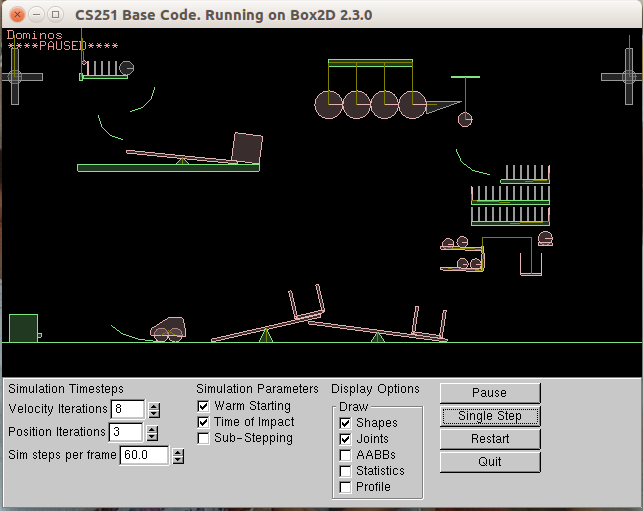
\includegraphics[width=0.7 \linewidth]{latex/box2d_prelim2.png}
	\end{figure} 
\end{columns} 
\end{frame}


\section{2. What are The technical Contributions?}
\begin{frame}
\frametitle{Why this will last?} 
\begin{itemize}
   \item This is the era of gaming!\pause
   \item Our product/project is a simulation! \pause
   \item It can be extended to a gaming simulation! \textbf{Kids can \emph{interact} with our product!} Play around with it! \pause
   \item Plus it's an \textbf{entertainer!}
\end{itemize} 
\end{frame}


\section{2.b What are the Challenges we faced?} 
\begin{frame}
\frametitle{Challenges} \begin{itemize}
   \item Firstly, we had to come up with some geek idea of a Rube Goldberg Machine! \pause
   \item Then, we had to find a way to create some elements like the button... \pause
   \item Make the saw cut the thread! 
\end{itemize}
\end{frame}


\section{3. How much effort we put in?}
\begin{frame}
\frametitle{Our passion} 
\begin{itemize}
   \item Our passion in a single liner!\pause
   \item \textbf{\emph{MAKE IT BETTER! :)}} \pause
   \item We work to improvise and give a better user-experience, satisfaction and entertainment!\pause
   \item No matter how much effort it takes!
\end{itemize} 
\end{frame}

\section{4. What we used from outside?}
\begin{frame}
\frametitle{Acknowledgement} 
\begin{itemize}
   \item This project was prepared under the able guidance of \emph{prof. Shrat Chandan}
   \item We used the \emph{"Box2D Package"} provided to us by \textbf{Software Systems Lab}.
   \item We surfed the internet and learnt from various sources, like 
\emph{"iforce2d", www.openGL.org, stackoverflow and various blogs} etc.
\end{itemize} 
\end{frame}




\end{document}
